\documentclass{article}
\usepackage{amsmath, array}
\usepackage{amssymb}
\usepackage{color, colortbl,xcolor,soul}
\usepackage{tikz}
\usepackage{tikz}

\begin{document}

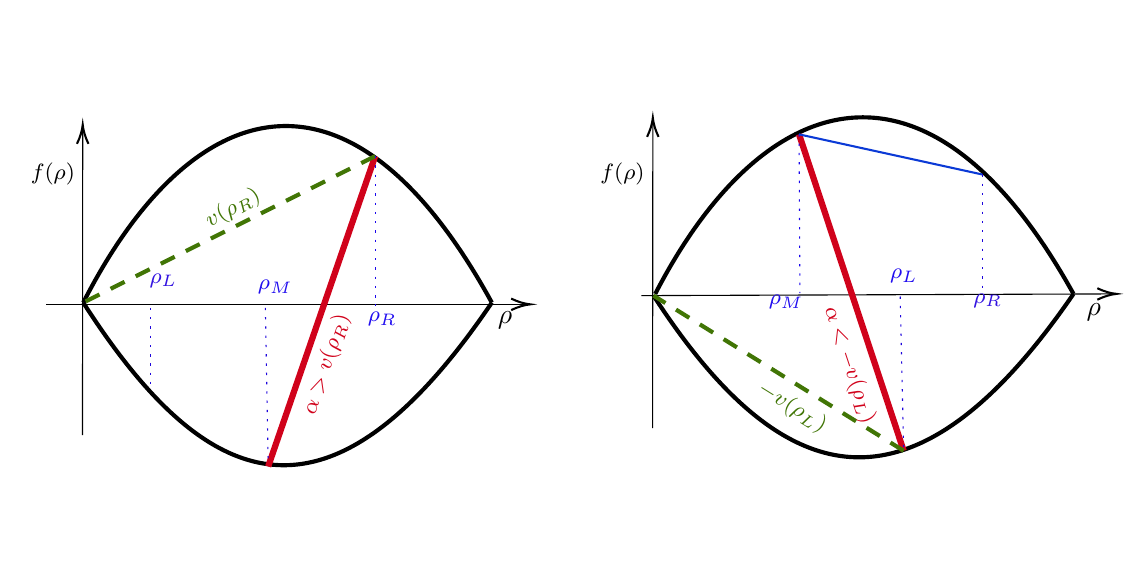
\begin{tikzpicture}[x=0.7pt,y=0.7pt,yscale=-0.9,xscale=0.9]

\draw    (26.83,149) -- (302.32,149) ;
\draw [shift={(304.32,149)}, rotate = 180] [color={rgb, 255:red, 0; green, 0; blue, 0 }  ][line width=0.75]    (10.93,-3.29) .. controls (6.95,-1.4) and (3.31,-0.3) .. (0,0) .. controls (3.31,0.3) and (6.95,1.4) .. (10.93,3.29)   ;
\draw [line width=1.5]    (47.93,148) .. controls (107.91,30.5) and (199.23,-3.5) .. (282.28,148) ;
\draw [line width=1.5]    (47.93,148) .. controls (118.93,258.5) and (189,285.5) .. (282.28,148) ;
\draw [color={rgb, 255:red, 208; green, 2; blue, 27 }  ,draw opacity=1 ][line width=2.25]    (154,242) -- (215.37,64) ;
\draw [color={rgb, 255:red, 65; green, 117; blue, 5 }  ,draw opacity=1 ][line width=1.5]  [dash pattern={on 5.63pt off 4.5pt}]  (215.37,64) -- (47.93,148) ;
\draw [color={rgb, 255:red, 30; green, 6; blue, 220 }  ,draw opacity=1 ] [dash pattern={on 0.84pt off 2.51pt}]  (152.39,151) -- (153.96,238) ;
\draw [color={rgb, 255:red, 30; green, 6; blue, 220 }  ,draw opacity=1 ] [dash pattern={on 0.84pt off 2.51pt}]  (86.26,151) -- (86.26,197) ;
\draw [color={rgb, 255:red, 26; green, 7; blue, 236 }  ,draw opacity=1 ] [dash pattern={on 0.84pt off 2.51pt}]  (215.37,64) -- (215.37,150) ;
\draw    (368,144) -- (638.5,143.01) ;
\draw [shift={(640.5,143)}, rotate = 539.79] [color={rgb, 255:red, 0; green, 0; blue, 0 }  ][line width=0.75]    (10.93,-3.29) .. controls (6.95,-1.4) and (3.31,-0.3) .. (0,0) .. controls (3.31,0.3) and (6.95,1.4) .. (10.93,3.29)   ;
\draw    (374.5,220) -- (374.63,44) ;
\draw [shift={(374.63,42)}, rotate = 450.04] [color={rgb, 255:red, 0; green, 0; blue, 0 }  ][line width=0.75]    (10.93,-3.29) .. controls (6.95,-1.4) and (3.31,-0.3) .. (0,0) .. controls (3.31,0.3) and (6.95,1.4) .. (10.93,3.29)   ;
\draw [line width=1.5]    (376,143) .. controls (436.68,25.5) and (531.9,-8.5) .. (615.91,143) ;
\draw [line width=1.5]    (375,144) .. controls (446.83,254.5) and (521.55,280.5) .. (615.91,143) ;
\draw [color={rgb, 255:red, 208; green, 2; blue, 27 }  ,draw opacity=1 ][line width=2.25]    (518.5,233) -- (458.5,51.5) ;
\draw [color={rgb, 255:red, 65; green, 117; blue, 5 }  ,draw opacity=1 ][line width=1.5]  [dash pattern={on 5.63pt off 4.5pt}]  (518.5,233) -- (375,144) ;
\draw [color={rgb, 255:red, 30; green, 6; blue, 220 }  ,draw opacity=1 ] [dash pattern={on 0.84pt off 2.51pt}]  (516.5,144.5) -- (518.5,233) ;
\draw [color={rgb, 255:red, 30; green, 6; blue, 220 }  ,draw opacity=1 ] [dash pattern={on 0.84pt off 2.51pt}]  (563.5,74.5) -- (563.5,141.5) ;
\draw [color={rgb, 255:red, 26; green, 7; blue, 236 }  ,draw opacity=1 ] [dash pattern={on 0.84pt off 2.51pt}]  (458.5,51.5) -- (459,142.5) ;
\draw    (47.5,224) -- (47.63,48) ;
\draw [shift={(47.63,46)}, rotate = 450.04] [color={rgb, 255:red, 0; green, 0; blue, 0 }  ][line width=0.75]    (10.93,-3.29) .. controls (6.95,-1.4) and (3.31,-0.3) .. (0,0) .. controls (3.31,0.3) and (6.95,1.4) .. (10.93,3.29)   ;
\draw [color={rgb, 255:red, 11; green, 58; blue, 214 }  ,draw opacity=1 ][line width=0.75]    (458.5,51.5) -- (563.5,74.5) ;

% Text Node
\draw (16.37,66.4) node [anchor=north west][inner sep=0.75pt]  [font=\footnotesize]  {$f( \rho )$};
% Text Node
\draw (284.28,151.4) node [anchor=north west][inner sep=0.75pt]    {$\rho $};
% Text Node
\draw (84.52,129.9) node [anchor=north west][inner sep=0.75pt]  [font=\footnotesize,color={rgb, 255:red, 50; green, 18; blue, 224 }  ,opacity=1 ]  {$\rho _{L}$};
% Text Node
\draw (209.71,151.9) node [anchor=north west][inner sep=0.75pt]  [font=\footnotesize,color={rgb, 255:red, 33; green, 13; blue, 239 }  ,opacity=1 ]  {$\rho _{R}$};
% Text Node
\draw (146.65,133.4) node [anchor=north west][inner sep=0.75pt]  [font=\footnotesize,color={rgb, 255:red, 33; green, 13; blue, 239 }  ,opacity=1 ]  {$\rho _{M}$};
% Text Node
\draw (169.58,211.76) node [anchor=north west][inner sep=0.75pt]  [font=\footnotesize,color={rgb, 255:red, 33; green, 13; blue, 239 }  ,opacity=1 ,rotate=-288.5,xslant=-0.08]  {$\textcolor[rgb]{0.82,0.01,0.11}{\alpha  >v}\textcolor[rgb]{0.82,0.01,0.11}{(}\textcolor[rgb]{0.82,0.01,0.11}{\rho }\textcolor[rgb]{0.82,0.01,0.11}{_{R}}\textcolor[rgb]{0.82,0.01,0.11}{)}$};
% Text Node
\draw (113.83,96.27) node [anchor=north west][inner sep=0.75pt]  [font=\footnotesize,color={rgb, 255:red, 33; green, 13; blue, 239 }  ,opacity=1 ,rotate=-330.58]  {$\textcolor[rgb]{0.25,0.46,0.02}{v}\textcolor[rgb]{0.25,0.46,0.02}{(}\textcolor[rgb]{0.25,0.46,0.02}{\rho }\textcolor[rgb]{0.25,0.46,0.02}{_{R}}\textcolor[rgb]{0.25,0.46,0.02}{)}$};
% Text Node
\draw (343.1,66.4) node [anchor=north west][inner sep=0.75pt]  [font=\footnotesize]  {$f( \rho )$};
% Text Node
\draw (622, 147.2) node [anchor=north west][inner sep=0.75pt]    {$\rho $};
% Text Node
\draw (556.94,141.4) node [anchor=north west][inner sep=0.75pt]  [font=\footnotesize,color={rgb, 255:red, 50; green, 18; blue, 224 }  ,opacity=1 ]  {$\rho _{R}$};
% Text Node
\draw (439.7,142.4) node [anchor=north west][inner sep=0.75pt]  [font=\footnotesize,color={rgb, 255:red, 33; green, 13; blue, 239 }  ,opacity=1 ]  {$\rho _{M}$};
% Text Node
\draw (509.27,127.4) node [anchor=north west][inner sep=0.75pt]  [font=\footnotesize,color={rgb, 255:red, 33; green, 13; blue, 239 }  ,opacity=1 ]  {$\rho _{L}$};
% Text Node
\draw (483.06,145.97) node [anchor=north west][inner sep=0.75pt]  [font=\footnotesize,color={rgb, 255:red, 33; green, 13; blue, 239 }  ,opacity=1 ,rotate=-71.57,xslant=-0.08]  {$\textcolor[rgb]{0.82,0.01,0.11}{\alpha < -v}\textcolor[rgb]{0.82,0.01,0.11}{(}\textcolor[rgb]{0.82,0.01,0.11}{\rho }\textcolor[rgb]{0.82,0.01,0.11}{_{L}}\textcolor[rgb]{0.82,0.01,0.11}{)}$};
% Text Node
\draw (438.9,189.08) node [anchor=north west][inner sep=0.75pt]  [font=\footnotesize,color={rgb, 255:red, 33; green, 13; blue, 239 }  ,opacity=1 ,rotate=-31.86]  {$\textcolor[rgb]{0.25,0.46,0.02}{-v}\textcolor[rgb]{0.25,0.46,0.02}{(}\textcolor[rgb]{0.25,0.46,0.02}{\rho }\textcolor[rgb]{0.25,0.46,0.02}{_{L}}\textcolor[rgb]{0.25,0.46,0.02}{)}$};
\end{tikzpicture}

\end{document}